\documentclass[12pt]{article}


%--------- Packages ----------------

\usepackage{graphicx} % Required for inserting images
\usepackage[a4paper,left=1in,right=1in,top=1in,bottom=1in]{geometry}
\usepackage{newtxtext} % If you need to use Time New Roman
\usepackage{newtxmath} % If you need to use Time New Roman
\usepackage[style=apa,backend=biber]{biblatex}
\usepackage[british]{babel}
\usepackage{csquotes}
\usepackage{bookmark}
\usepackage{setspace}
\usepackage{fancyhdr}
\usepackage[font=footnotesize,justification=centering]{caption}
\usepackage{hyperref}
\usepackage{float}
\usepackage{setspace}

%--------- Set Up ------------------
\setstretch{1.5}
\pagestyle{fancy}
\fancypagestyle{plain}{%
  \renewcommand{\headrulewidth}{0pt}%
  \fancyhf{}}


% --- title insert (check title.tex for more)----------

\title{How do computers actually compute?} % TITLE HERE 
\author{ Ethan Garcia  \\ Joshua Sundararaman  \\   Jimmy Chen \\}

%-------- Document -----------------

\begin{document}


\begin{titlepage}
    \newcommand{\HRule}{\rule{\linewidth}{0.5mm}} % Defines a new command for the horizontal lines, change thickness here

    \center
    \textsc{\large CSCI2500 Final Project}\\[1.5cm]

    \makeatletter
    \rule{\linewidth}{0.2 mm} \\[0.4 cm]
    {\huge\bfseries \@title \par} \
    \rule{\linewidth}{0.2 mm} \\[1.0 cm]
    \emph{Team ID:}\\ 49\\[1cm]
    \emph{Authors:}\\
    \@author
    \vspace{1cm}
    \emph{Course Coordinator:}\\
    Konstatin Kuzmin\\
    \vspace{1cm}
    \makeatother
    {\large \today}\\[2cm] % Date, change the \today to a set date if you want to be precise
    \vfill % Fill the rest of the page with whitespace
\end{titlepage}

\fancyhf{}
\setlength{\headheight}{33pt}
\fancyhead[L]{\nouppercase{\leftmark}}
\fancyhead[R]{Team ID: 49}
\fancyfoot[R]{ \bf\thepage\ \rm }
\fancyfoot[L]{\emph{CSCI2500 Final Project} }

\newpage
\tableofcontents
\newpage
\section{Requirements}
\begin{itemize}
    \item \textbf{Bit Width} - 16-bit
    \item \textbf{Main Memory Size} - 64Ki bytes
    \item \textbf{Main Memory Organization} - 8Ki x 8
    \item \textbf{Max number of bits to be used by L1 cache:} - 40,000
    \item \textbf{Additional Addressing Mode} - Indirect
\end{itemize}
\subsubsection{Components Needed}
\begin{center}
    \begin{tabular}{|p{5cm}|p{10cm}|}
        \hline
        \textbf{Component}               & \textbf{Function}                                                                                                                                 \\
        \hline
        AC or Accumulator                & Intermediate data is stored within the AC                                                                                                         \\
        \hline
        PC or Program Counter            & As the name suggests it counts the current position of the code, each line has its own address; PC needs to be incremented after each instruction \\
        \hline
        MAR or Memory Access Register    & Stores or fetches the ’data’ at the given address                                                                                                 \\
        \hline
        MBR or Memory Buffer Register    & Stores the data when being transferred                                                                                                            \\
        \hline
        IR or Instruction Register       & Stores the instruction word of the currently executing instruction                                                                                \\
        \hline
        ALU or Arithmetic and Logic Unit & Performs arithmetic and Boolean operations                                                                                                        \\
        \hline
        Main memory                      & Stores data and instructions                                                                                                                      \\
        \hline
    \end{tabular}
\end{center}

\newpage
\section{Design 1}\
\subsection{Instruction Set Architecture}
\begin{center}
    \begin{tabular}{|p{3cm}|p{3cm}|}
        \hline
        \textbf{Opcode} & \textbf{Operation} \\
        \hline
        \verb|1000|     & \verb|ADD|         \\
        \hline
        \verb|1001|     & \verb|HALT|        \\
        \hline
        \verb|1010|     & \verb|LOAD|        \\
        \hline
        \verb|1011|     & \verb|STORE|       \\
        \hline
        \verb|1100|     & \verb|CLEAR|       \\
        \hline
        \verb|1101|     & \verb|SKIP|        \\
        \hline
        \verb|1110|     & \verb|JUMP|        \\
        \hline
    \end{tabular}
\end{center}

\subsection{Components}
\subsubsection{ALU}
\textbf{Overview:}\\
The ALU is a crucial component in a computer's architecture responsible for performing arithmetic and logic operations.
In this 16-bit ALU, the operations include addition, subtraction, bitwise AND, bitwise OR, bitwise XOR, bitwise NOT for A,
bitwise NOT for B, and clearing the output. The \verb|ALU_Sel| input determines the operation to be performed.\\
\textbf{Inputs:}
\begin{itemize}
    \item A and B: 16-bit operands on which operations are performed
    \item \verb|ALU_Sel|: 4-bit input that specifies the operation to be executed.
\end{itemize}
\textbf{Outputs:}
\begin{itemize}
    \item \verb|ALU_Out|: 16-bit output that stores the result of the operation.
    \item \verb|CarryOut|: 1-bit output that stores the carry bit of the operation.
\end{itemize}
\textbf{Internal Signals:}
\begin{itemize}
    \item \verb|ALU_Result|: 16-bit register storing the result of the selected operation.
    \item \verb|tmp|: 17-bit wire used to calculate the carry-out during addition.
\end{itemize}
\textbf{Operation Execution:}
\begin{itemize}
    \item The \verb|tmp| wire is used to calculate the sum of A and B along with the carry bit (if any) during addition.
    \item The carry-out (\verb|CarryOut|) is extracted from the 17th bit of \verb|tmp|.
    \item The result of the selected operation is determined using a case statement based on the value of \verb|ALU_Sel|.
\end{itemize}
\textbf{Supported Operations:}
\begin{itemize}
    \item \verb|0000|: Addition
    \item \verb|0001|: Subtraction
    \item \verb|0010|: Bitwise AND
    \item \verb|0011|: Bitwise OR
    \item \verb|0100|: Bitwise XOR
    \item \verb|0101|: Bitwise NOT for A
    \item \verb|0110|: Bitwise NOT for B
    \item \verb|0111|: Clear output
\end{itemize}
\pagebreak
\textbf{Code:}
\begin{center}
    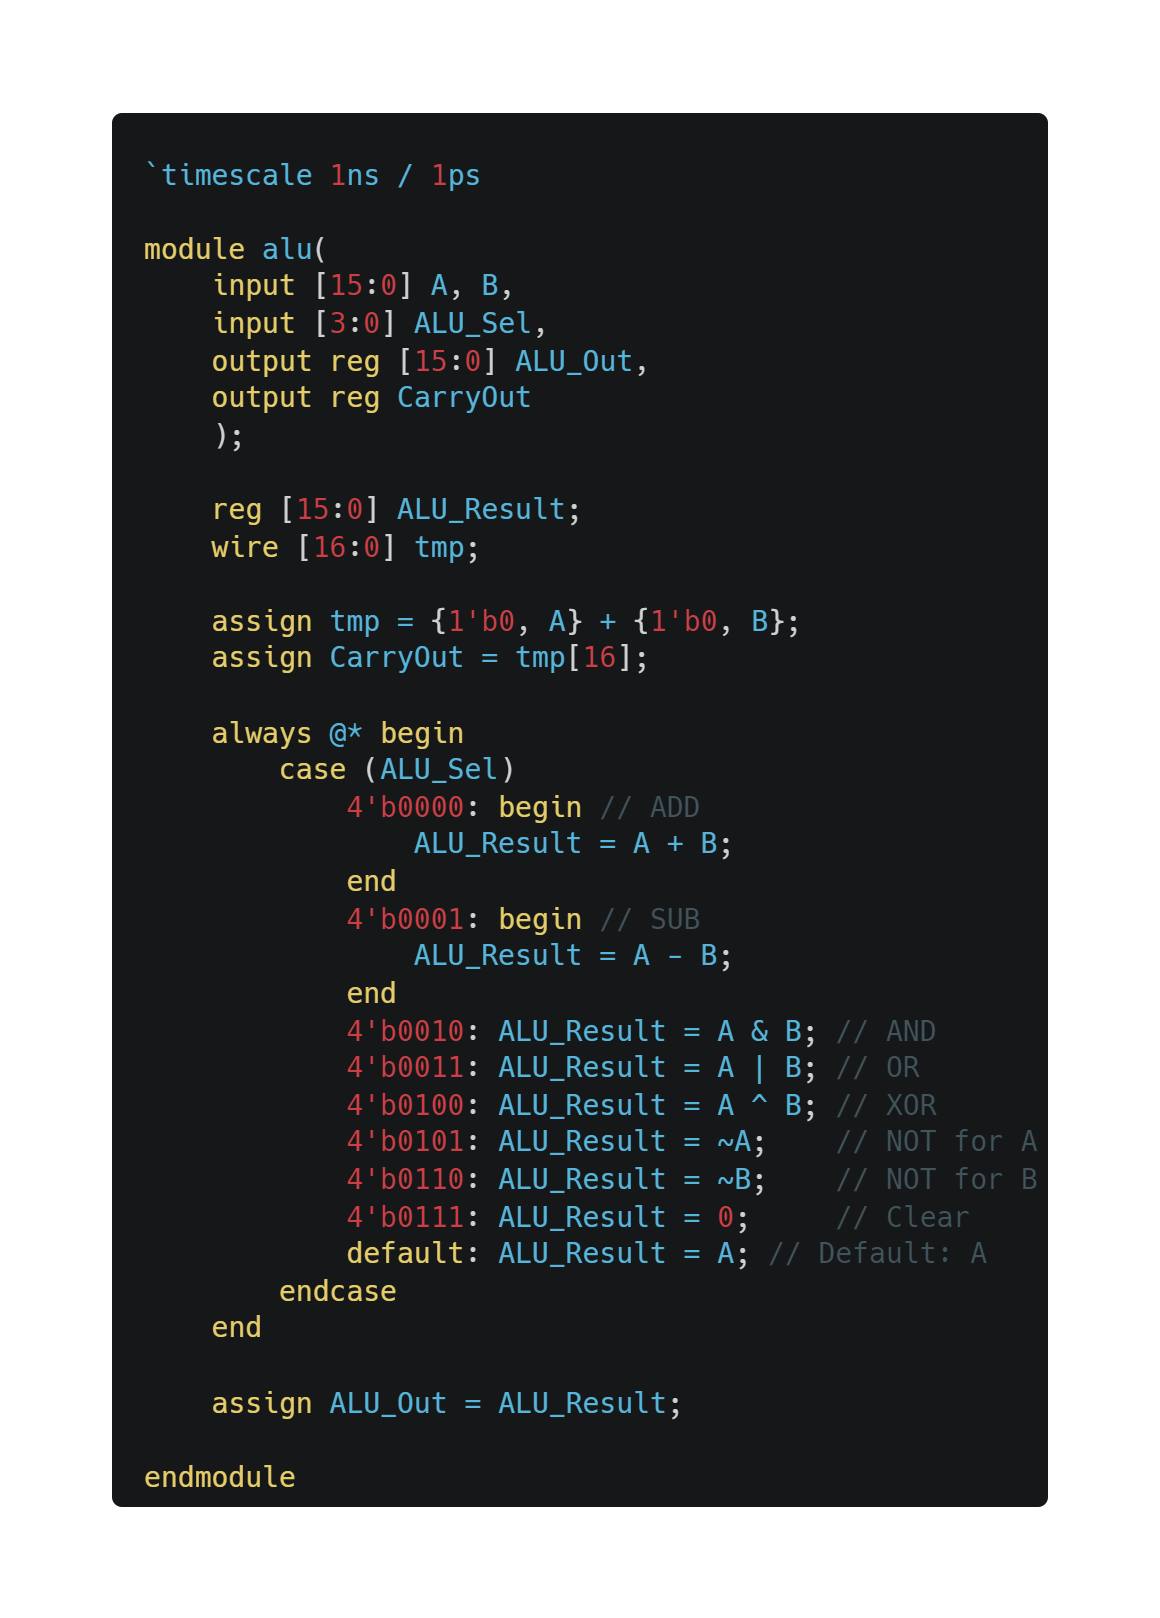
\includegraphics[scale=0.25]{images/alu.png}
\end{center}
\begin{enumerate}
    \item The addition operation is performed using both the assign statement and within the case statement to illustrate two different methods.
    \item The case statement handles all possible operation cases based on the \verb|ALU_Sel| input.
    \item The default case is set to pass the value of A when an unrecognized operation is specified.
    \item The \verb|ALU_Out| is assigned the value of \verb|ALU_Result| to provide the result of the selected operation.
\end{enumerate}
\pagebreak
\textbf{Testbench:}
\begin{center}
    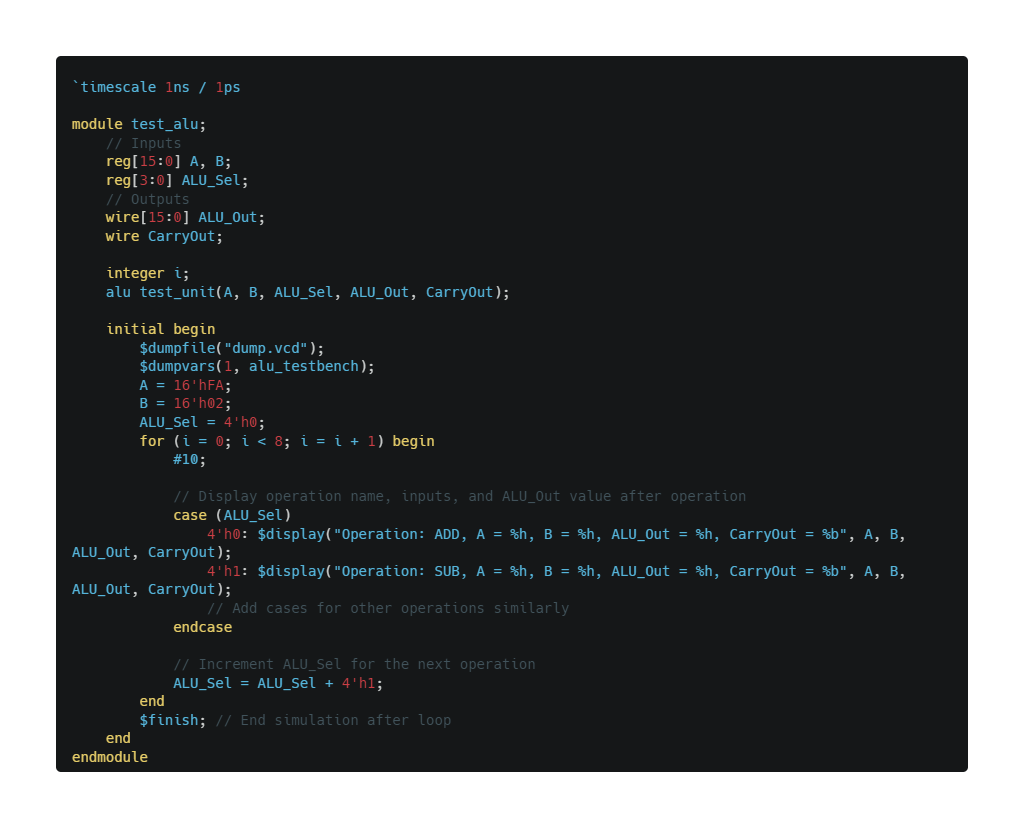
\includegraphics[width=\linewidth]{images/alu_tb.png}
\end{center}
Console Output:
\begin{verbatim}
Operation: ADD, A = 00fa, B = 0002, ALU_Out = 00fc, CarryOut = 0
Operation: SUB, A = 00fa, B = 0002, ALU_Out = 00f8, CarryOut = 0
\end{verbatim}
EPWave:
\begin{center}
    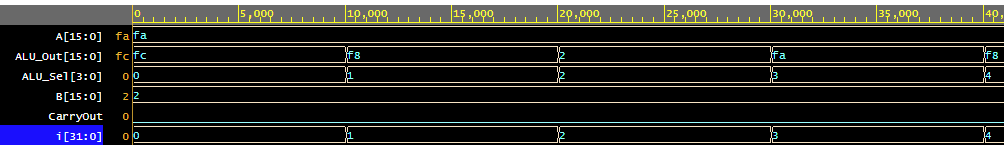
\includegraphics[width=\linewidth]{images/alu_tb_wave.png}
\end{center}
\newpage
\subsubsection{Decoder}
\textbf{Overview:}\\
A decoder is a digital circuit that converts an n-bit binary code into a $2^n$ line output. In this 16-bit decoder, the input in is an n-bit binary code,
and the output out is a $2^n$-bit vector where only one bit is set to '1' based on the input value.\\
\textbf{Inputs:}\\
\verb|in|: An n-bit input that represents the binary code to be decoded.
\textbf{Outputs:}\\
\verb|out|: A $2^n$-bit vector where only the bit corresponding to the input value is set to '1'.\\
\textbf{Parameters:}\\
\verb|ENCODE_WIDTH|: A parameter that determines the width of the input (in) and the number of outputs (out).
\textbf{Local Parameters:}\\
\verb|latency|: A local parameter set to 1, indicating the latency of the assignment operation.
\textbf{Operation Execution:}\\
The assignment statement uses the shift-left (\verb|<<|) operator to set the bit at the position specified by the value of in to '1'. All other bits remain '0'.\\
\textbf{Code:}
\begin{center}
    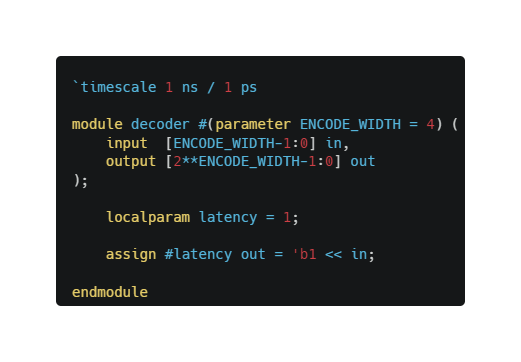
\includegraphics[width=\linewidth]{images/decoder.png}
\end{center}
\begin{enumerate}
    \item The localparam statement defines a local parameter latency set to 1, indicating a single time unit of delay for the assignment operation.
    \item The assign statement performs a bitwise shift operation (<<) to set the output bit corresponding to the binary value of in to '1'.
          This effectively decodes the binary input into a one-hot representation.
    \item The parameter \verb|ENCODE_WIDTH| determines the width of the input and the number of output bits. If \verb|ENCODE_WIDTH| is 4, then the output vector will have $2^4 = 16$ bits.
\end{enumerate}
\pagebreak
\textbf{Testbench:}
\begin{center}
    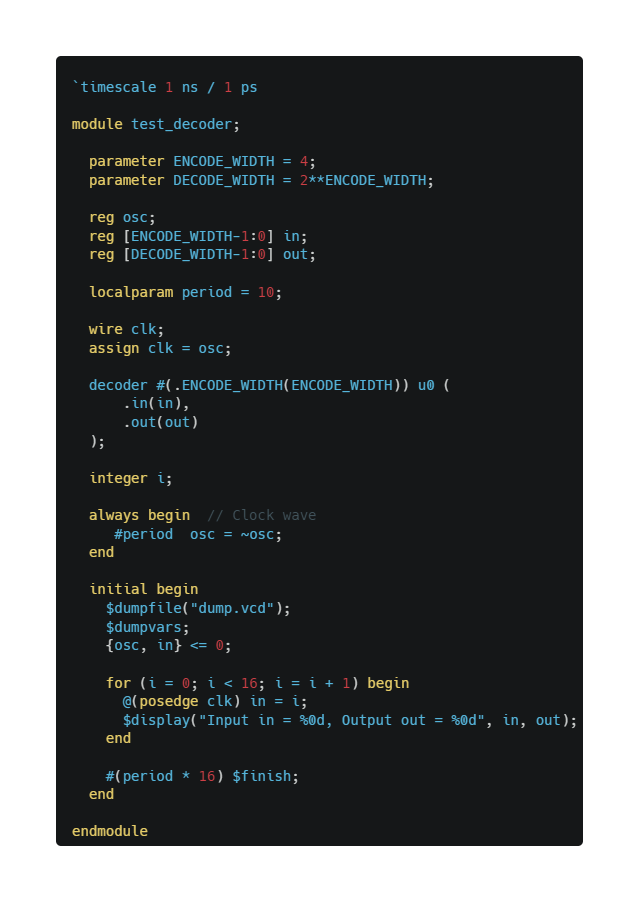
\includegraphics[width=\linewidth]{images/decoder_tb.png}
\end{center}
Console Output:
\begin{verbatim}
Input in = 0, Output out = 1
Input in = 1, Output out = 1
Input in = 2, Output out = 2
Input in = 3, Output out = 4
Input in = 4, Output out = 8
Input in = 5, Output out = 16
Input in = 6, Output out = 32
Input in = 7, Output out = 64
Input in = 8, Output out = 128
Input in = 9, Output out = 256
Input in = 10, Output out = 512
Input in = 11, Output out = 1024
Input in = 12, Output out = 2048
Input in = 13, Output out = 4096
Input in = 14, Output out = 8192
Input in = 15, Output out = 16384
\end{verbatim}
EPWave:
\begin{center}
    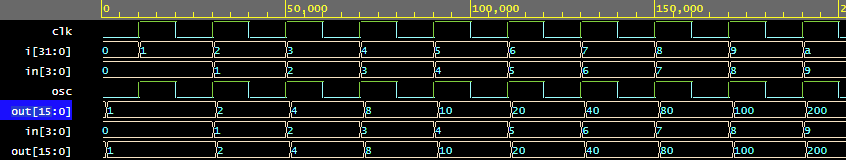
\includegraphics[width=\linewidth]{images/decoder_tb_wave.png}
\end{center}
\pagebreak
\subsubsection{Ram}
\textbf{Overview:}\\
A single-port synchronous RAM module is designed to store and retrieve data based on the address provided. It is synchronous, meaning that data is read and written on clock edges. This RAM module is parameterized with options for address width (\verb|ADDR_WIDTH|), data width (\verb|DATA_WIDTH|), and length (\verb|LENGTH|) of the memory.\\
\textbf{Parameters:}\\
\begin{itemize}
    \item \verb|ADDR_WIDTH|: Parameter specifying the width of the address bus.
    \item \verb|DATA_WIDTH|: Parameter specifying the width of the data bus.
    \item \verb|LENGTH|: Parameter specifying the length of the memory, calculated as $2^(\text{ADDR\_WIDTH})$.
\end{itemize}
\textbf{Inputs:}\\
\begin{itemize}
    \item \verb|clk|: Clock input for synchronous operation.
    \item \verb|addr|: Address bus indicating the location in memory.
    \item \verb|data|: Bidirectional data bus for read and write operations.
    \item \verb|cs|: Chip select signal.
    \item \verb|we|: Write enable signal.
    \item \verb|oe|: Output enable signal.
\end{itemize}
\textbf{Outputs:}\\
\begin{itemize}
    \item \verb|tmp_data|: Temporary storage for data during read operations.
    \item \verb|mem|: Memory array to store data.
\end{itemize}
\textbf{Write Operation:}\\
On the positive edge of the clock (posedge clk), if the chip select (cs) and write enable (we) signals are active, the data at the specified address (addr) is updated with the input data.\\
\textbf{Read Operation}:\\
On the negative edge of the clock (negedge clk), if the chip select (cs) is active and write enable (we) is inactive, the data at the specified address (addr) is loaded into the temporary storage (\verb|tmp_data|).\\
\textbf{Data Output:}\\
The assign statement determines the output data based on chip select (cs), output enable (oe), and write enable (we). If the chip select and output enable are active while write enable is inactive, the output data is set to the temporary data (\verb|tmp_data|). Otherwise, it is set to 'bz' (high-impedance).\\
\textbf{Code:}
\begin{center}
    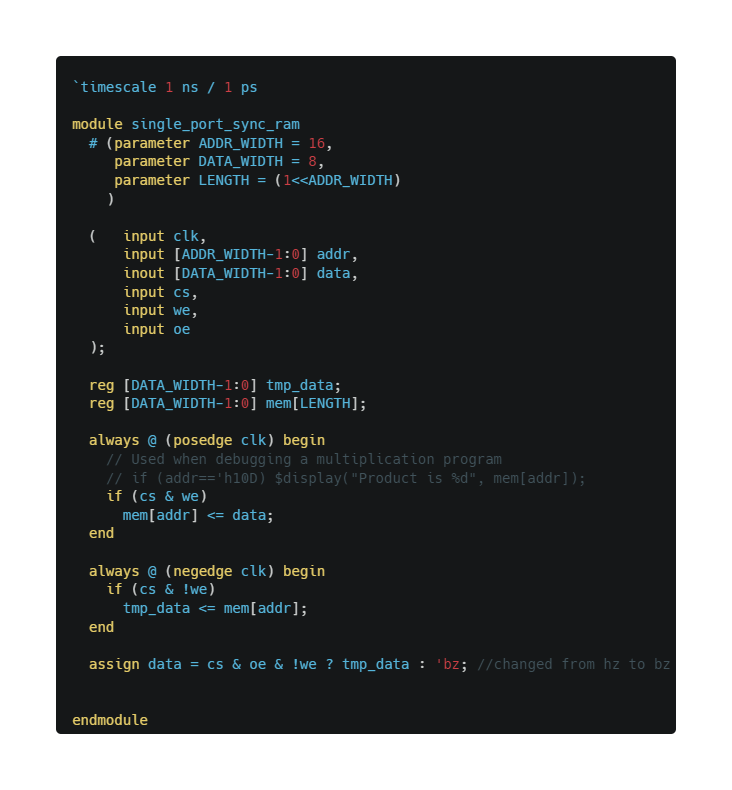
\includegraphics[scale=0.5]{images/ram.png}
\end{center}
\pagebreak
\textbf{Testbench:}
\begin{center}
    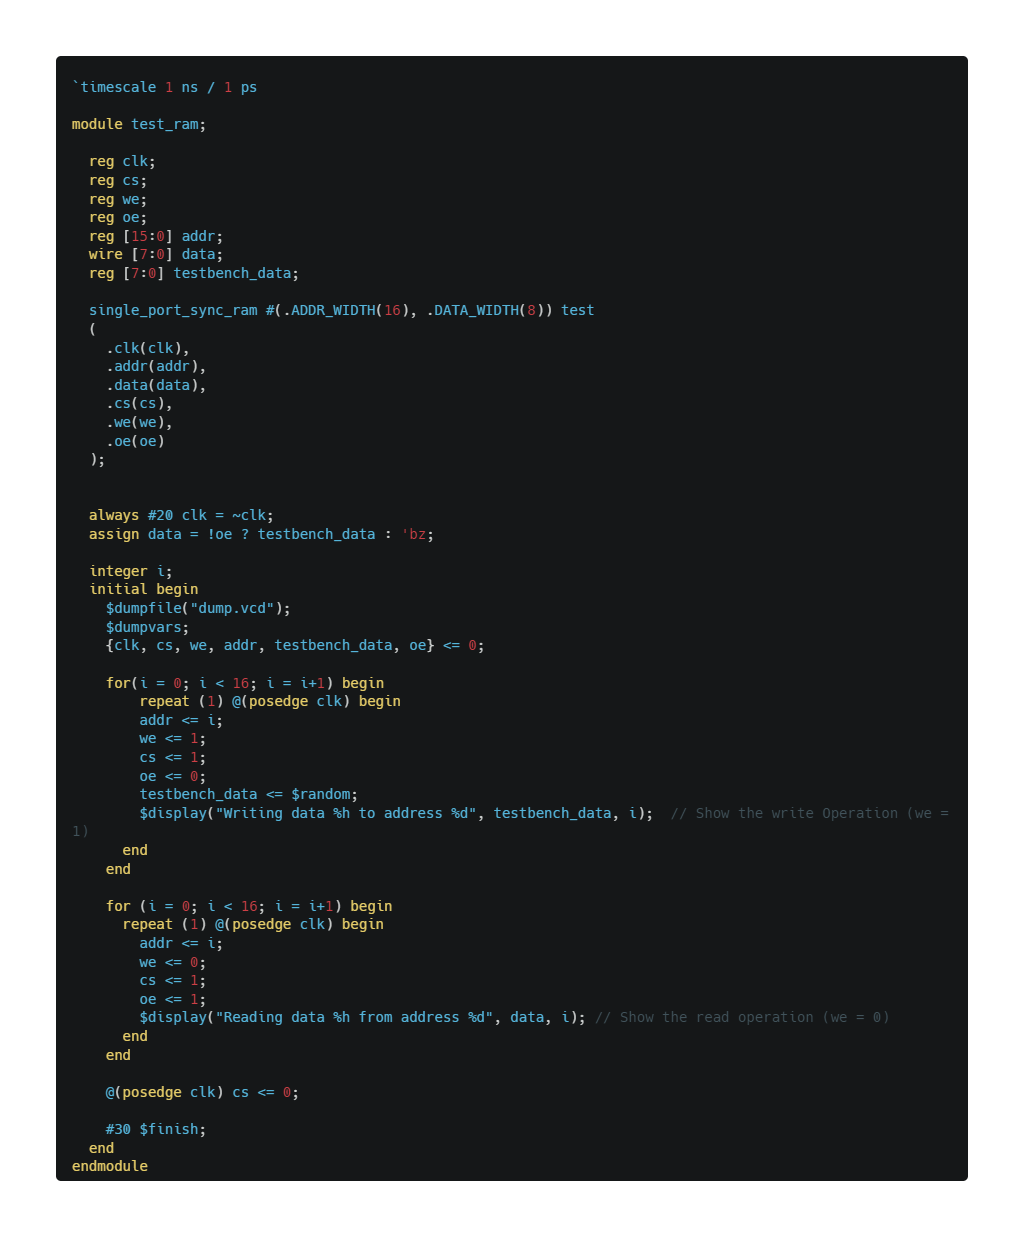
\includegraphics[scale=0.5]{images/ram_tb.png}
\end{center}
Console Output:
\begin{verbatim}
Writing data 00 to address           0
Writing data 24 to address           1
Writing data 81 to address           2
Writing data 09 to address           3
Writing data 63 to address           4
Writing data 0d to address           5
Writing data 8d to address           6
Writing data 65 to address           7
Writing data 12 to address           8
Writing data 01 to address           9
Writing data 0d to address          10
Writing data 76 to address          11
Writing data 3d to address          12
Writing data ed to address          13
Writing data 8c to address          14
Writing data f9 to address          15
Reading data c6 from address           0
Reading data 24 from address           1
Reading data 81 from address           2
Reading data 09 from address           3
Reading data 63 from address           4
Reading data 0d from address           5
Reading data 8d from address           6
Reading data 65 from address           7
Reading data 12 from address           8
Reading data 01 from address           9
Reading data 0d from address          10
Reading data 76 from address          11
Reading data 3d from address          12
Reading data ed from address          13
Reading data 8c from address          14
Reading data f9 from address          15
\end{verbatim}
EPWave:
\begin{center}
    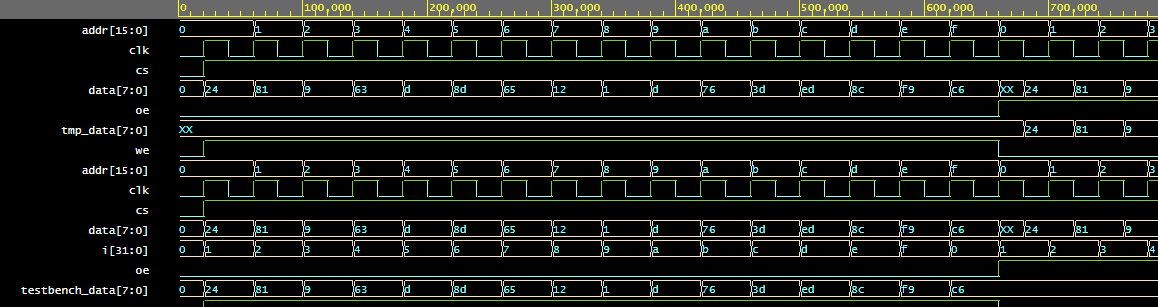
\includegraphics[width=\linewidth]{images/ram_tb_wave.png}
\end{center}
\newpage
\subsubsection{Large Ram}
\textbf{Overview:}\\
This module is designed for a 16-bit system and includes a larger single-port synchronous RAM composed of multiple smaller RAMs. It uses a decoder to generate chip select signals for each smaller RAM module based on a subset of the address bits.
\textbf{Parameters:}
\begin{itemize}
    \item \verb|ADDR_WIDTH|: Parameter specifying the width of the address bus.
    \item \verb|DATA_WIDTH|: Parameter specifying the width of the data bus.
    \item \verb|DATA_WIDTH_SHIFT|: Parameter determining the shift amount for splitting the data bus into two parts.
\end{itemize}
\textbf{Inputs:}
\begin{itemize}
    \item \verb|clk|: Clock input for synchronous operation.
    \item \verb|addr|: Address bus indicating the location in memory.
    \item \verb|data|: Bidirectional data bus for read and write operations.
    \item \verb|cs|: Chip select signal.
    \item \verb|we|: Write enable signal.
    \item \verb|oe|: Output enable signal.
\end{itemize}
\textbf{Internal Wires:}\\
\verb|cs|: 4-bit wire representing chip select signals generated by the decoder.\\
\textbf{Decoder:}\\
An instance of the decoder module is used to decode a subset of address bits (\verb|addr[ADDR_WIDTH-1:ADDR_WIDTH-2]|) into chip select signals (\verb|cs[3:0]|).\\
\textbf{Smaller RAM Modules:}\\
Four instances each of smaller single-port synchronous RAM modules (\verb|u00, u01, ..., u31|) are instantiated to form the larger RAM. Each instance corresponds to a different subset of address bits and has its own chip select signal (\verb|cs[0], cs[1], cs[2], cs[3]|).\\
\pagebreak
\textbf{Code:}
\begin{center}
    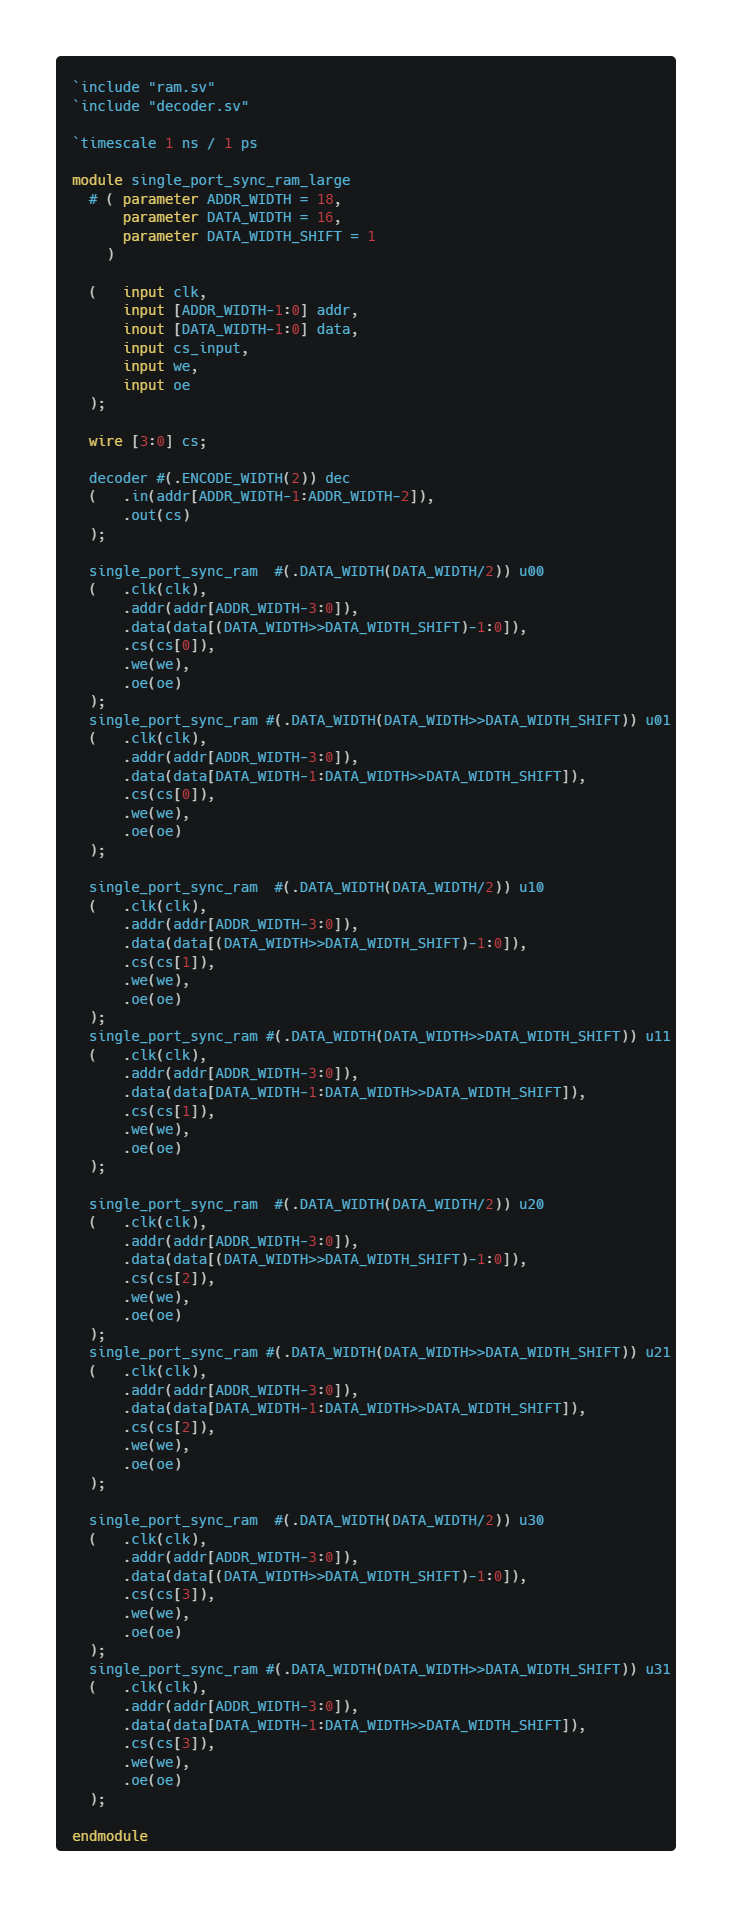
\includegraphics[scale=0.38]{images/ram_large.png}
\end{center}
\textbf{Testbench:}
\begin{center}
    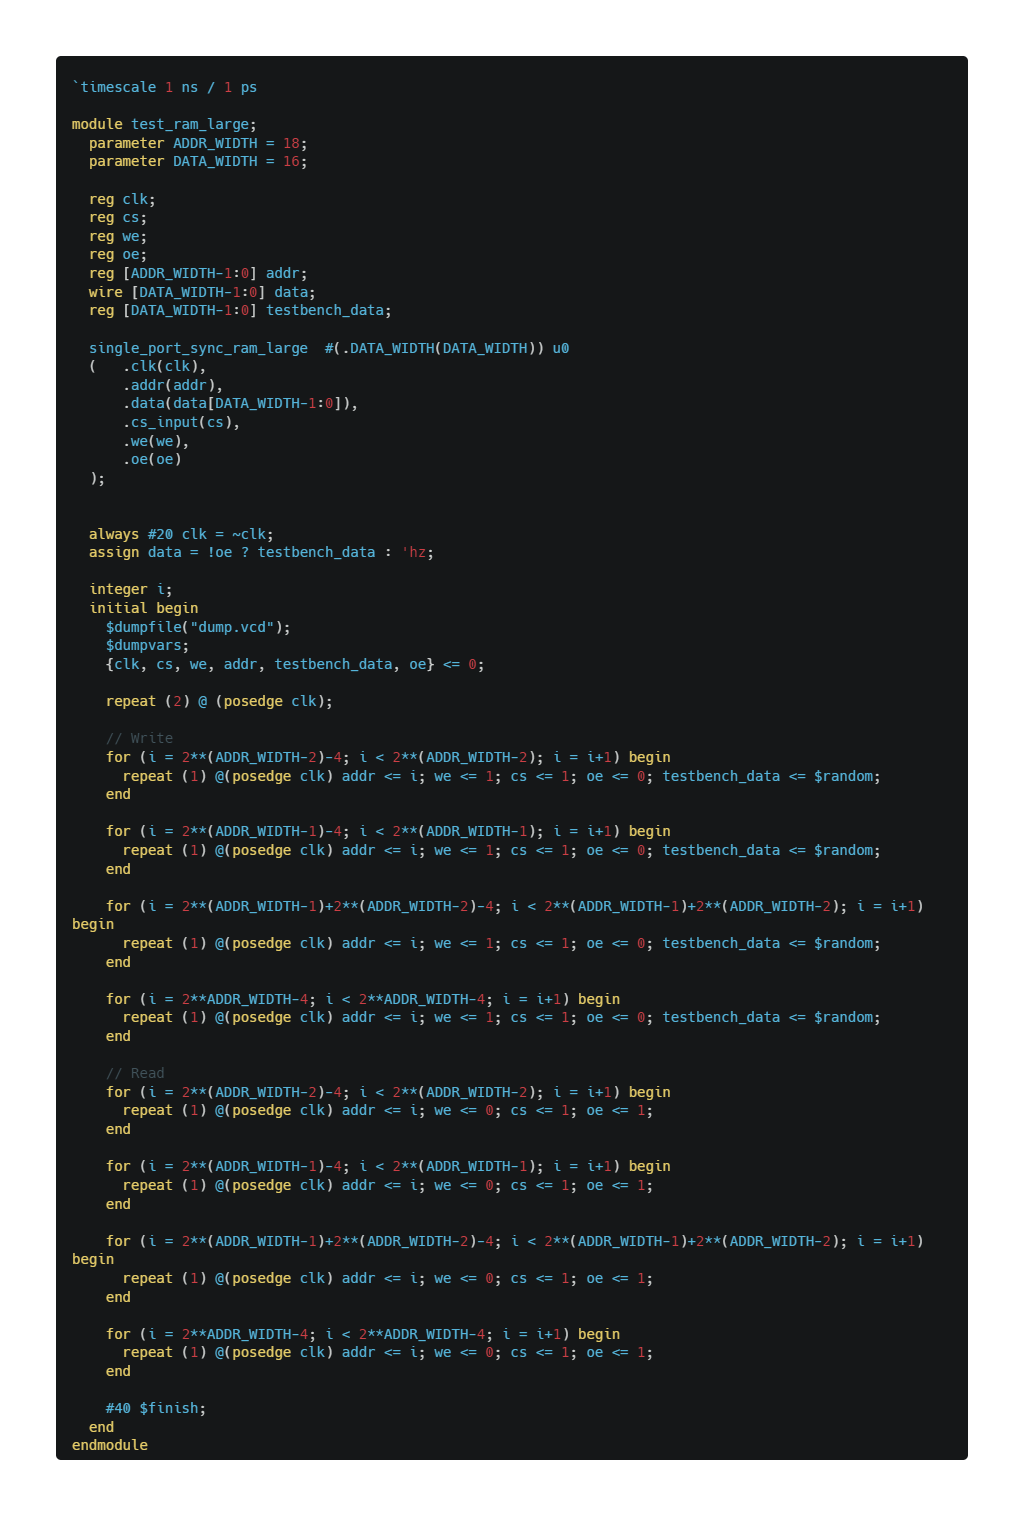
\includegraphics[scale=0.3]{images/ram_large_tb.png}
\end{center}
EPWave:
\begin{center}
    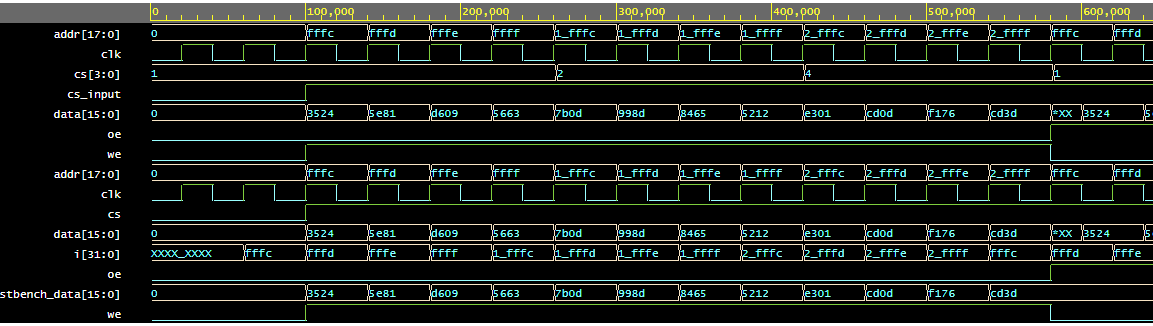
\includegraphics[scale = 0.5]{images/ram_large_tb_wave.png}
\end{center}
\pagebreak
\subsubsection{CPU}
\textbf{Overview:}\\
The module represents a basic 16-bit CPU with a simple instruction set architecture. The CPU fetches, decodes, and executes instructions stored in memory. The memory is implemented using the \verb|single_port_sync_ram_large module|, and arithmetic/logic operations are performed using the alu module. The CPU executes a Fibonacci sequence calculation as an example program.
\textbf{Parameters:}\\
\begin{itemize}
    \item \verb|ADDR_WIDTH|: Parameter specifying the width of the address bus.
    \item \verb|DATA_WIDTH|: Parameter specifying the width of the data bus.
\end{itemize}
\textbf{Clock Generation:}
The module includes a clock (clk) derived from an oscillator (osc). The clock waveform is generated with a period of 10 time units, using a toggling osc signal.
\textbf{Memory (RAM):}
An instance of the \verb|single_port_sync_ram_large| module is instantiated to represent the memory (RAM) for storing program instructions and data. The RAM is 16 bits wide, and the address width is 18 bits.
\textbf{ALU (Arithmetic Logic Unit):}
An instance of the alu module (alu16) is instantiated to perform arithmetic and logic operations. It takes two 16-bit inputs (A and B) and produces a 16-bit output (\verb|ALU_Out|). The ALU selection (\verb|ALU_Sel|) is controlled by the CPU instructions.
\textbf{Registers:}
Several registers are defined for the CPU, including:
\begin{itemize}
    \item MAR (Memory Address Register)
    \item data (Data Bus)
    \item \verb|testbench_data| (Testbench Data)
    \item A and B (ALU Inputs)
    \item \verb|ALU_Out| (ALU Output)
    \item PC (Program Counter)
    \item IR (Instruction Register)
    \item MBR (Memory Buffer Register)
    \item AC (Accumulator)
\end{itemize}

\textbf{Instruction Execution Loop:}
The CPU includes an initial block that initializes the clock waveform and sets up the program for Fibonacci sequence calculation.
A loop is implemented for instruction execution, where instructions are fetched, decoded, and executed in a sequential manner.
The program uses a simple instruction set, where each instruction is a 16-bit word.

\textbf{Instruction Set:}
The instruction set includes operations such as load, store, add, subtract, logical AND, logical OR, halt, skip, jump, and clear accumulator.\\
\newpage
\textbf{Code:}
\begin{center}
    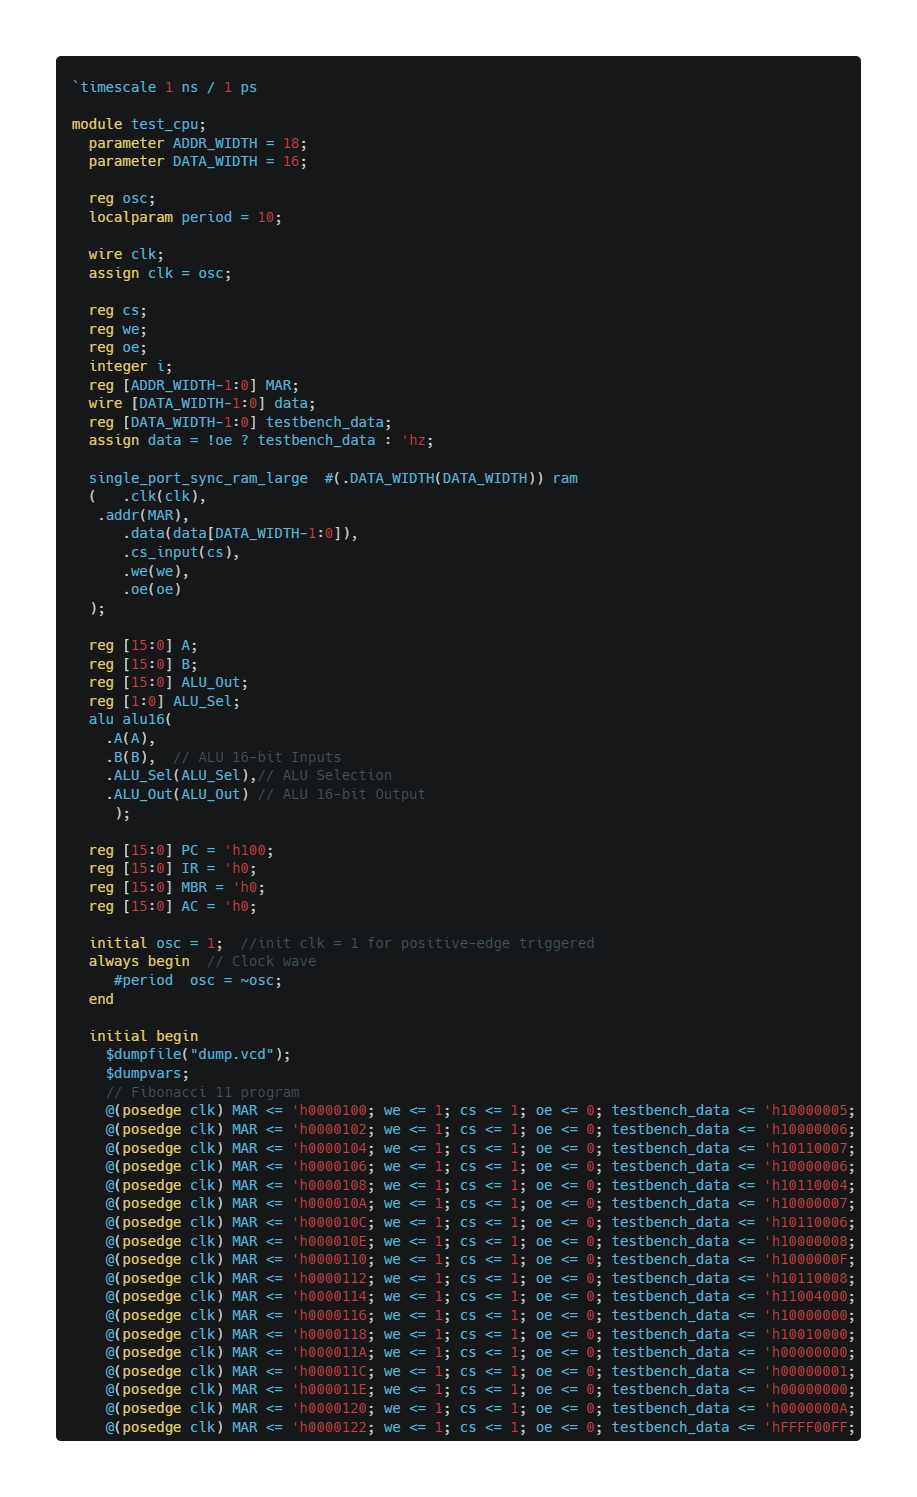
\includegraphics[scale=0.45]{images/design1_1.png}
    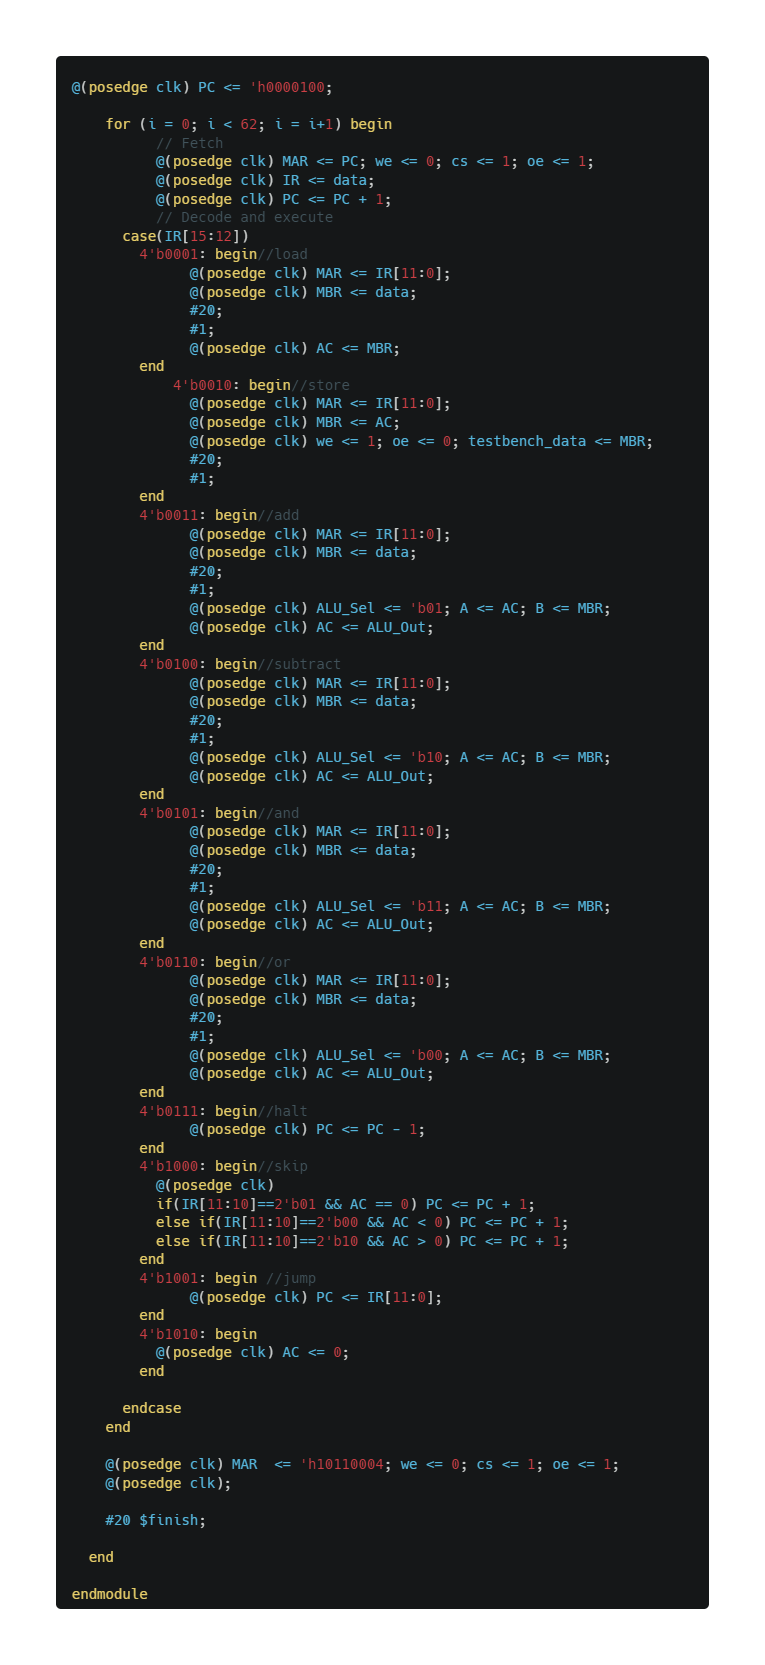
\includegraphics[scale=0.4]{images/design1_2.png}
\end{center}
\pagebreak
\textbf{Testbench:}
EPWave:
\begin{center}
    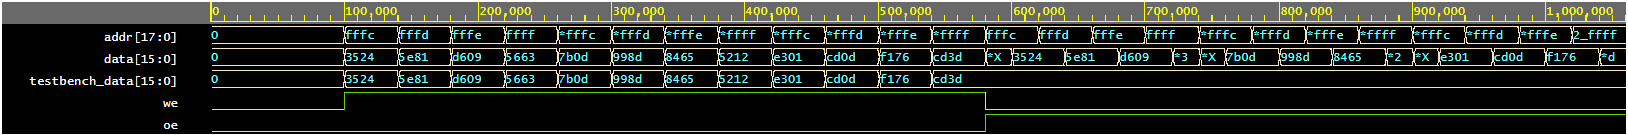
\includegraphics[width=\linewidth]{images/design1a_wave.png}
\end{center}

\section{Design 1a}
CPU with indirect addressing.
\begin{center}
    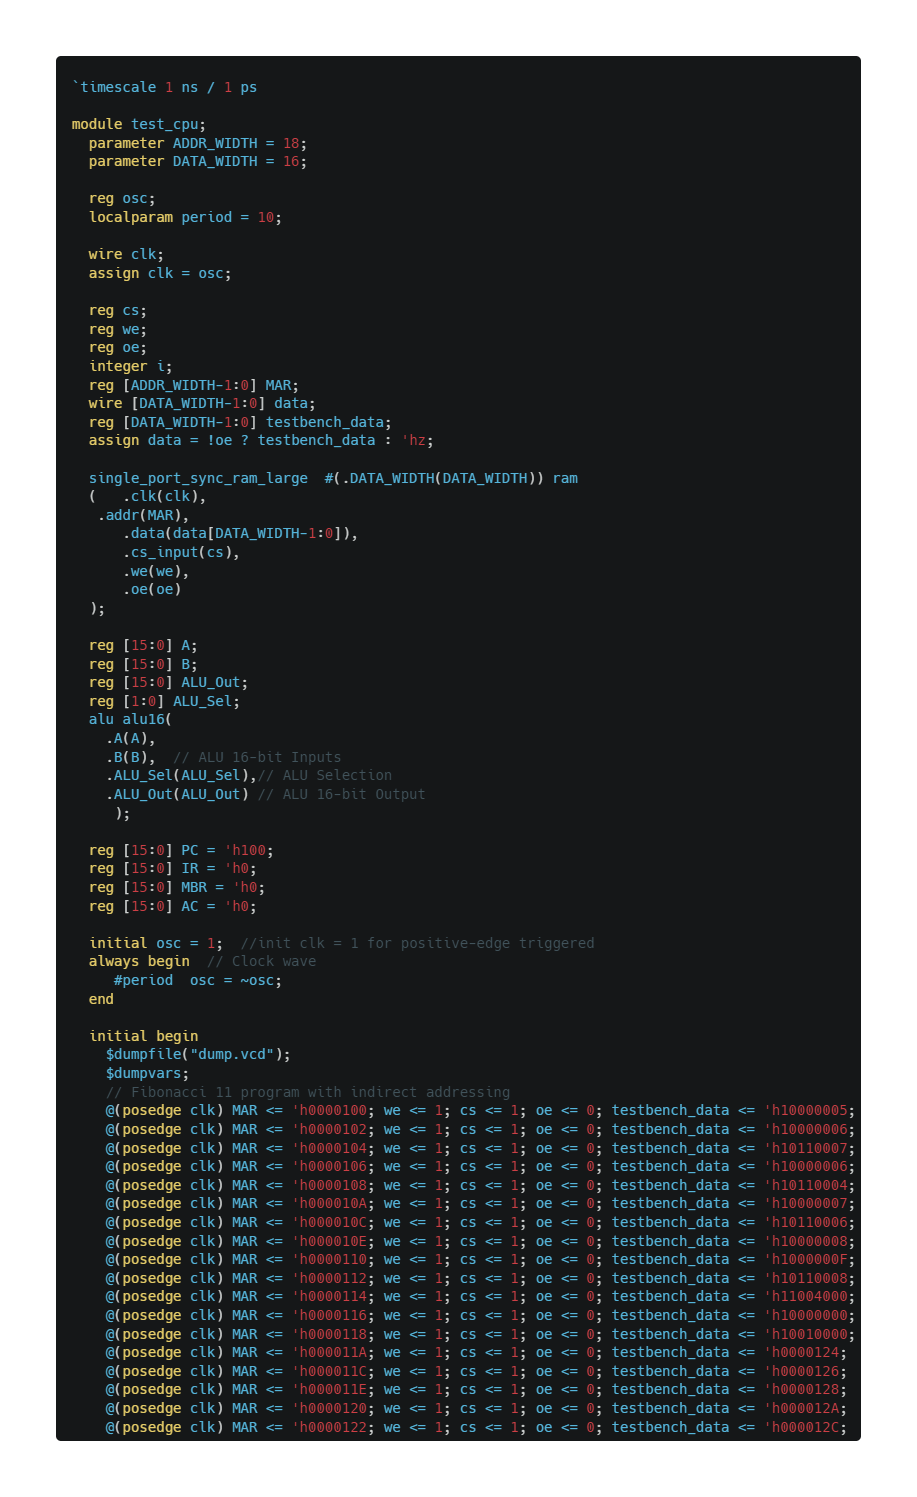
\includegraphics[scale=0.35]{images/a_1.png}
\end{center}
\begin{center}
    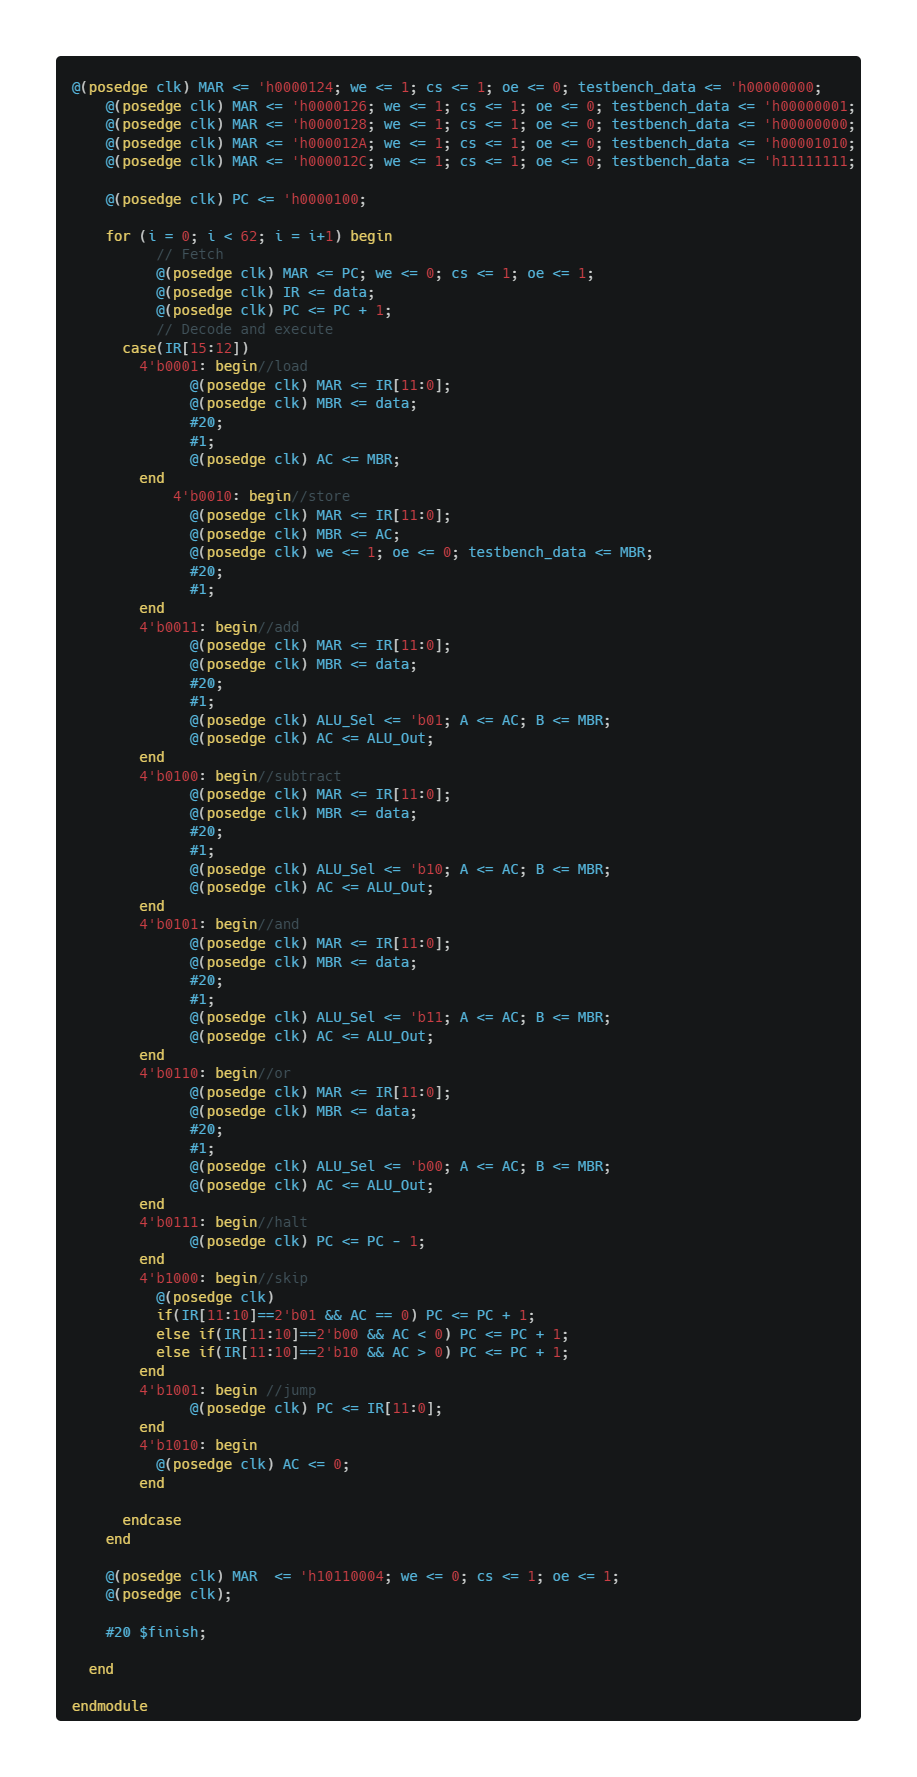
\includegraphics[scale=0.35]{images/a_2.png}
\end{center}


\newpage
\section{Design 1b}
\begin{center}
    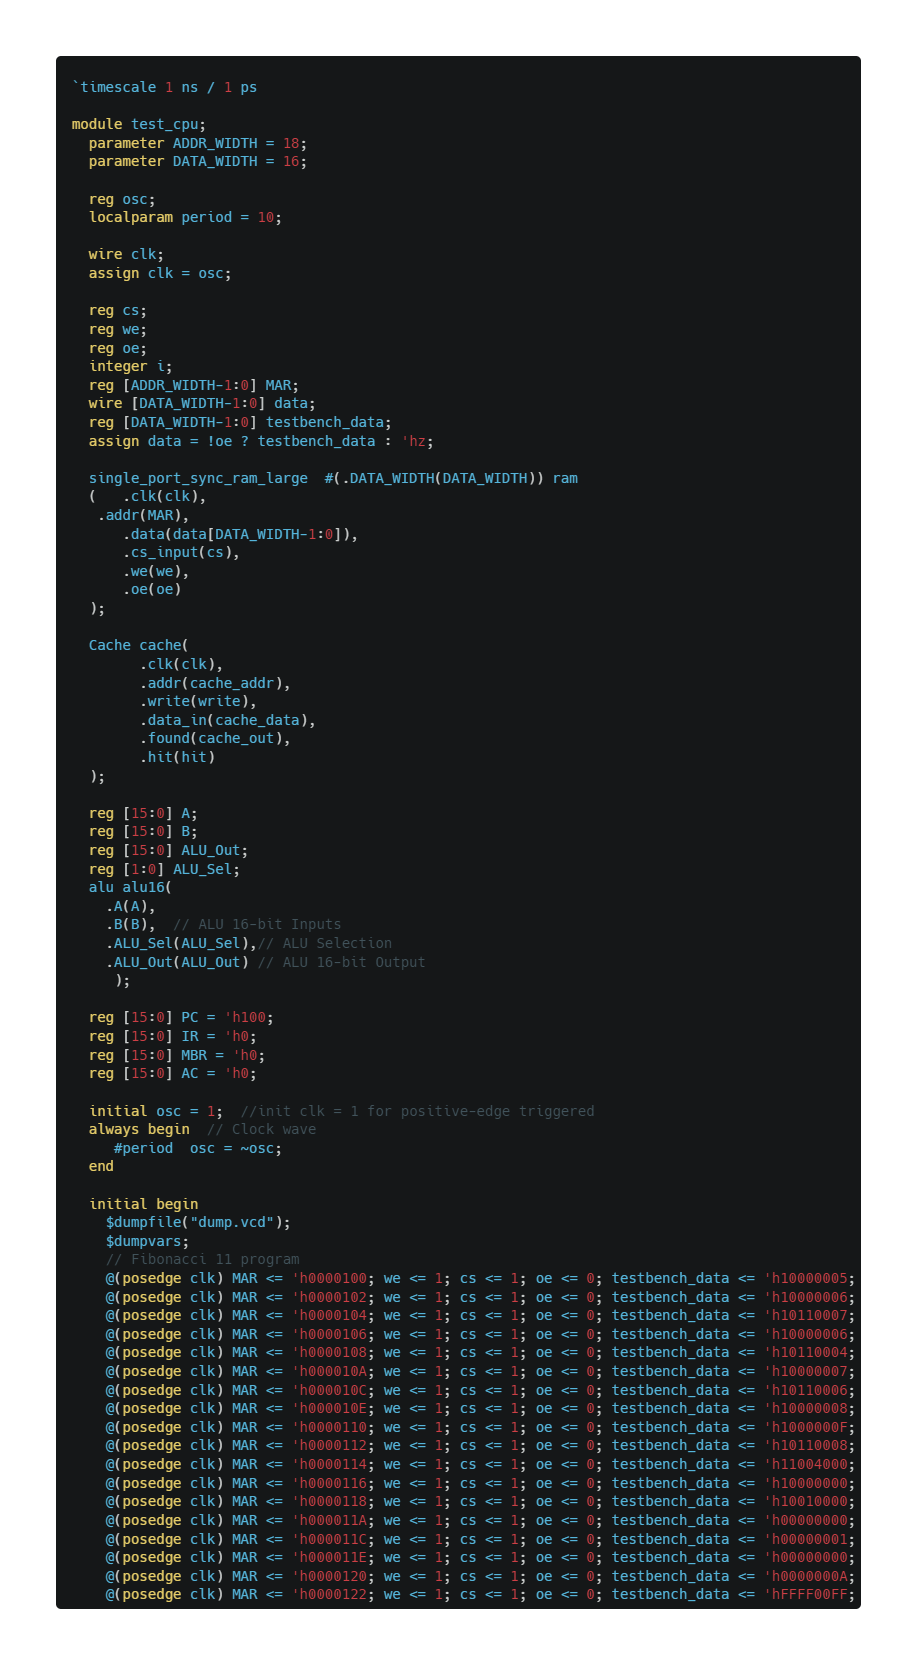
\includegraphics[scale=0.35]{images/b_1.png}
\end{center}
\begin{center}
    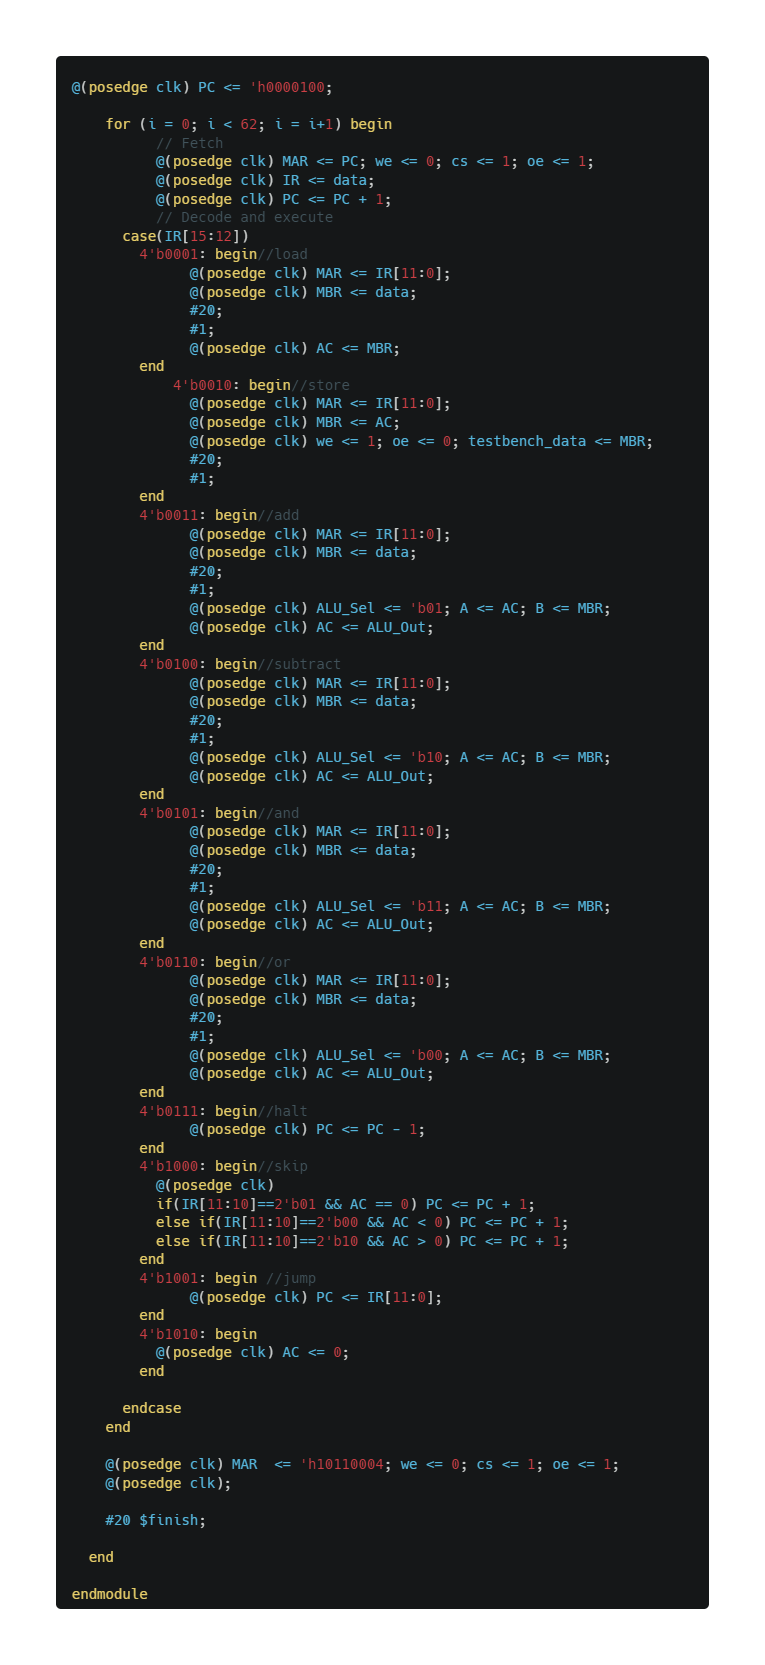
\includegraphics[scale=0.35]{images/b_2.png}
\end{center}
\subsection{Data Cache Implementation}
In the updated CPU design, a data cache has been seamlessly integrated using a dedicated module called `Cache`. This cache module acts as an intermediary between the CPU and the main memory (`ram` module), offering a faster data access mechanism for frequently used information. The cache is equipped with input and output ports, such as `clk` (clock), `addr` (address), `write` (write enable), `\verb|data_in|` (input data), `found` (cache hit signal), and `hit` (hit line). The CPU leverages the cache by fetching data through it, and the resultant information is stored in the `data` signal for subsequent processing. The cache implementation includes hit detection logic (`found` signal) to determine whether the requested data is present in the cache, optimizing data access by reducing latency associated with memory retrieval.\\

Within the CPU execution loop, the `data` signal is dynamically assigned based on the presence or absence of a cache hit. If a cache hit is detected, the data is directly sourced from the cache (`\verb|data_in|`). On the other hand, in the event of a cache miss, the CPU fetches the required data from the main memory (`ram` module). Additionally, the cache module facilitates write operations back to memory, controlled by the `write` signal. Overall, the integration of the data cache enhances the CPU's performance by minimizing memory access times and streamlining the retrieval of frequently accessed data, contributing to improved overall system efficiency.


\newpage
\section{Testbench}
\subsection{Fibonacci F11}
\textbf{Code:}\\
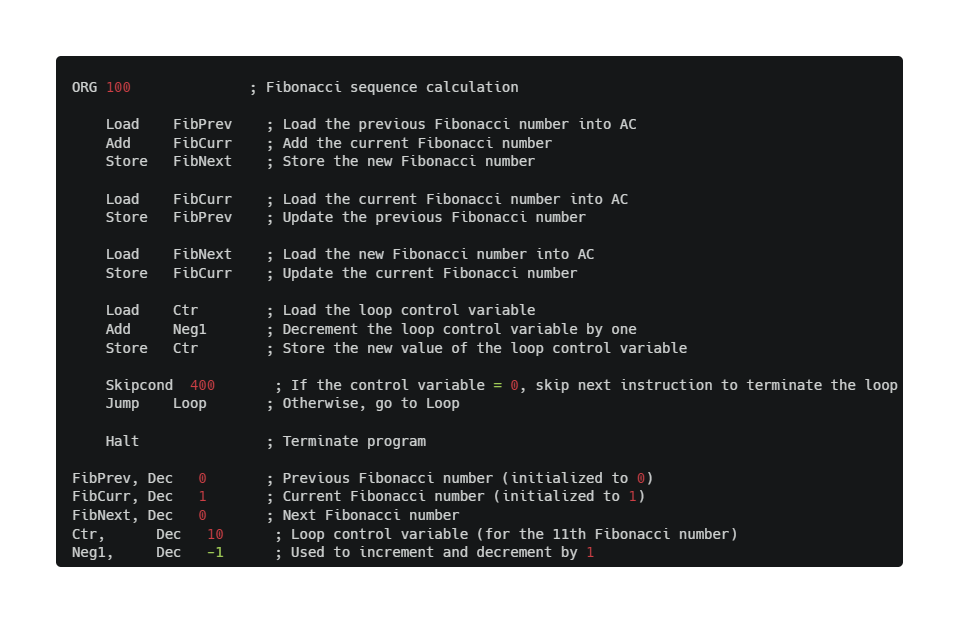
\includegraphics[width=\linewidth]{images/fibonacci.png}
\textbf{Machine Code:}\\
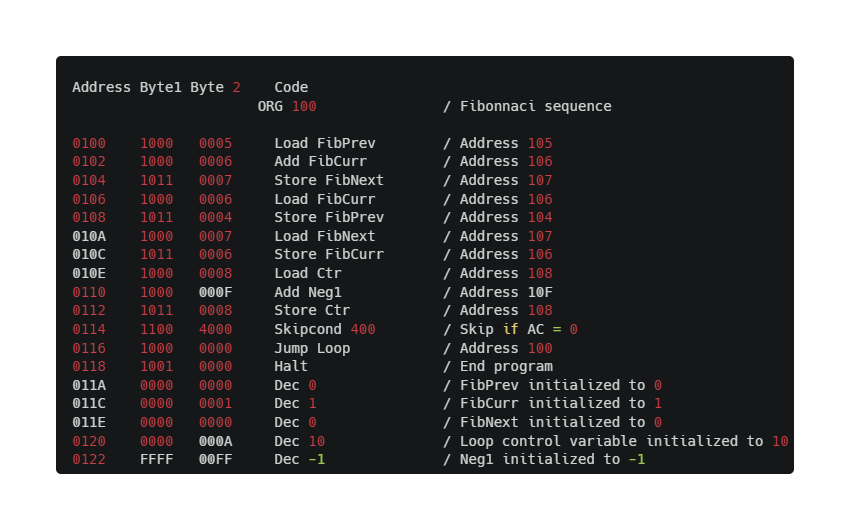
\includegraphics[width=\linewidth]{images/fibonacci_machine.png}

\noindent To translate the assembly code down into machine code, we used the opcode from our ISA for each
instruction to assign them an address. Then we used the address to assign each instruction a binary value.\\

\noindent For example, using the first four lines of the assembly code this is how they were translated:
\begin{enumerate}
    \item \verb|ORG 100|: This instruction sets the origin of the program to address 100. The machine code at address 100 is 1000 0000 (1000 for the opcode "ORG" and 0000 for the operand "100").
    \item \verb|Load FibPrev|: In the provided assembly language, the Load instruction is represented by the opcode 1000. The operand 0005 represents the address of the variable FibPrev. Therefore, the machine code for this line is 1000 0005 (1000 for "Load" and 0005 for the operand).
    \item \verb|Add FibCurr|: The Add instruction is represented by the opcode 1000, and the operand 0006 corresponds to the address of the variable FibCurr. Thus, the machine code is 1000 0006.
    \item \verb|Store FibNext|: The Store instruction is represented by the opcode 1011, and the operand 0007 corresponds to the address of the variable FibNext. Therefore, the machine code is 1011 0007.
\end{enumerate}
This process is repeated for each line of the assembly code, with each mnemonic and operand being translated into the corresponding machine code.

\end{document}
